% questions.tex —— 1977 年·宁夏卷 · 题目内容片段（无答案）
% 由 tools/generate_projects.py 依来源总账自 1977/1977_数学真题_宁夏_试题.md 生成，勿手改（改源 MD 后重跑）


\gkpart{数学试卷（宁夏卷）}

\begin{gktip}
\textbf{来源说明}：本题面依据固定源 PDF《宁夏1977年高考数学试题解》第 1—6 页（书籍页码 46—51）逐题转录。固定源是题面与解答连续出现的材料，不是无答案试卷；配套答案与解析对照源解答独立复算，\textbf{不是官方标准答案}。原卷文理合卷、同题异分：第一大题每小题文科 6 分、理科 5 分，第二大题文科 14 分、理科 12 分，第三、四大题均文科 13 分、理科 12 分，第五大题理科 14 分、文科不作；末尾附加题 2 题满分 20 分，在 100 分之外计入总分。
\textbf{题号说明}：原卷按大题编排、不设全卷连续题号。本库按全卷连续编号转录：原卷第一大题的 10 个小题转录为第 1—10 题，第二大题的两个选作题转录为第 11、12 题（原卷注明「下列两题只选作一题」），第三、四、五大题依次转录为第 13、14、15 题；小问编号照录，未增删任何题干内容。
\end{gktip}

\par\medskip

\begin{question}
\gkti{1}\textbf{（文科 6 分，理科 5 分）} 计算

\nopagebreak[4]
\[
\left(2\frac79\right)^{\frac12}+3^{-2}-\left(\frac13\right)^0.
\]

\end{question}
\begin{question}
\gkti{2}\textbf{（文科 6 分，理科 5 分）} 化简：

\nopagebreak[4]
\[
\sqrt{12}-\sqrt{48}-3\sqrt3.
\]

\end{question}
\begin{question}
\gkti{3}\textbf{（文科 6 分，理科 5 分）} 分解因式：

\nopagebreak[4]
\[
mx^2+2mxy+my^2.
\]

\end{question}
\begin{question}
\gkti{4}\textbf{（文科 6 分，理科 5 分）} 解方程：

\nopagebreak[4]
\[
2x^2-3x+1=0.
\]

\end{question}
\begin{question}
\gkti{5}\textbf{（文科 6 分，理科 5 分）} 已知 $\operatorname{Sin}\alpha=\dfrac35$（$\alpha$ 是锐角），求：

（1） $\operatorname{Cos}\alpha$；

（2） $\operatorname{tg}\alpha$。

\end{question}
\begin{question}
\gkti{6}\textbf{（文科 6 分，理科 5 分）} 不查表求：

\nopagebreak[4]
\[
\operatorname{Lg}8+\operatorname{Lg}125-\operatorname{Lg}1.
\]

\end{question}
\begin{question}
\gkti{7}\textbf{（文科 6 分，理科 5 分）} 求经过点 $(4,-4)$ 和原点的直线方程。

\end{question}
\begin{question}
\gkti{8}\textbf{（文科 6 分，理科 5 分）} 解不等式：$(x+1)(x-2)<0$。

\end{question}
\begin{question}
\gkti{9}\textbf{（文科 6 分，理科 5 分）} 求

\nopagebreak[4]
\[
\frac12+\frac14+\frac18+\frac1{16}+\cdots+\frac{1}{2^{10}}.
\]

\Needspace{0.4\textheight}
\end{question}
\begin{question}
\gkti{10}\textbf{（文科 6 分，理科 5 分）} 已知：在 $\triangle ABC$ 中，$\angle B=60^\circ$，$AD\perp BC$，$AD=3$，$AC=5$。求：$BC$，$AB$。
\nopagebreak[4]
\begin{center}% 1977 年宁夏卷第 10 题：三角形 ABC（A 在上方），AD 为 BC 边上的垂线，D 为垂足（按源卷第 2 页布局）
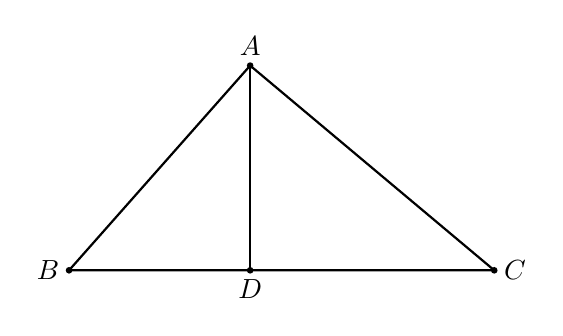
\begin{tikzpicture}[scale=1.0]
  \coordinate (A) at (2.3,2.6);
  \coordinate (B) at (0,0);
  \coordinate (C) at (5.4,0);
  \coordinate (D) at (2.3,0);
  \draw[thick] (B)--(C)--(A)--cycle;
  \draw[thick] (A)--(D);
  \fill (A) circle (1.2pt) node[above] {$A$};
  \fill (B) circle (1.2pt) node[left] {$B$};
  \fill (C) circle (1.2pt) node[right] {$C$};
  \fill (D) circle (1.2pt) node[below] {$D$};
\end{tikzpicture}
\end{center}
\nopagebreak[4]
\Needspace{0.4\textheight}
\end{question}
\begin{question}
\gkti{11}\textbf{（文科 14 分，理科 12 分）} 在 $\triangle ABC$ 中，已知 $a=\sqrt2$，$A=45^\circ$，$B=60^\circ$，求 $C$、$b$、$c$ 及面积 $\triangle$。
\nopagebreak[4]
\begin{center}% 1977 年宁夏卷第 11 题：三角形 ABC（C 在上方），三边分别标注 a（BC 边）、b（CA 边）、c（AB 边）（按源卷第 2 页布局）
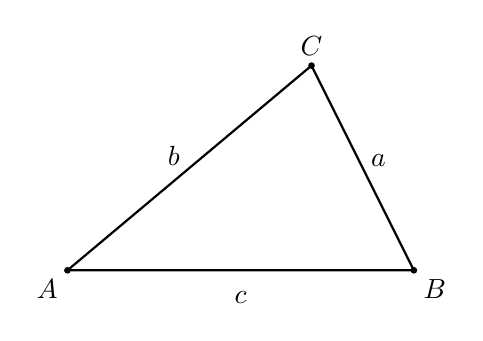
\begin{tikzpicture}[scale=1.0]
  \coordinate (A) at (0,0);
  \coordinate (B) at (4.4,0);
  \coordinate (C) at (3.1,2.6);
  \draw[thick] (A)--(B)--(C)--cycle;
  \fill (A) circle (1.2pt) node[below left] {$A$};
  \fill (B) circle (1.2pt) node[below right] {$B$};
  \fill (C) circle (1.2pt) node[above] {$C$};
  \node at (1.35,1.45) {$b$};
  \node at (3.95,1.4) {$a$};
  \node at (2.2,-0.35) {$c$};
\end{tikzpicture}
\end{center}
\nopagebreak[4]
\end{question}
\begin{question}
\gkti{12}\textbf{（文科 14 分，理科 12 分）} 求与直线 $x+y=1$ 相切于点 $(2,-1)$，并且圆心在直线 $y=-2x$ 上圆的方程。

\Needspace{0.4\textheight}
\end{question}
\begin{question}
\gkti{13}\textbf{（文科 13 分，理科 12 分）} 已知圆内接三角形 $ABC$，$AB$、$BC$ 上的高 $CE$、$AD$ 相交于 $H$，$AD$ 延长线与 $\overset{\frown}{BC}$ 交于 $F$。求证：$HD=FD$。
\nopagebreak[4]
\begin{center}% 1977 年宁夏卷第 13 题：圆内接三角形 ABC，AB、BC 边上的高 CE、AD 相交于 H，
% AD 延长线交弧 BC 于 F，连线 FC 为虚线；角 1 在 B、角 2 在 C、角 3 在 H、角 4 在 F（按源卷第 3 页布局）
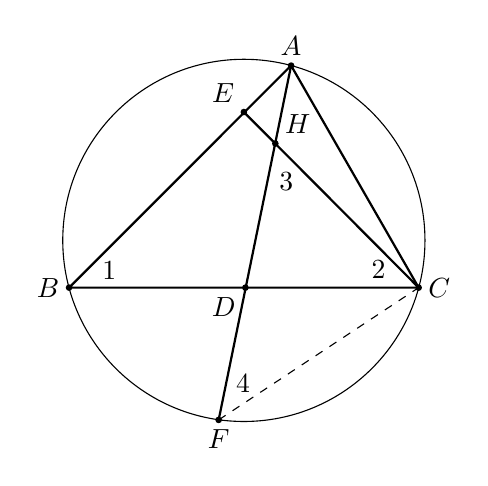
\begin{tikzpicture}[scale=1.0]
  \draw (2.6,2.1) circle (2.3);
  \coordinate (A) at (3.2,4.32);
  \coordinate (B) at (0.38,1.5);
  \coordinate (C) at (4.82,1.5);
  \coordinate (D) at (2.62,1.5);
  \coordinate (E) at (2.6,3.73);
  \coordinate (H) at (3.0,3.33);
  \coordinate (F) at (2.28,-0.18);
  \draw[thick] (A)--(B)--(C)--cycle;
  \draw[thick] (A)--(F);
  \draw[thick] (C)--(E);
  \draw[dashed] (F)--(C);
  \fill (A) circle (1.2pt) node[above] {$A$};
  \fill (B) circle (1.2pt) node[left] {$B$};
  \fill (C) circle (1.2pt) node[right] {$C$};
  \fill (D) circle (1.2pt) node[below left] {$D$};
  \fill (E) circle (1.2pt) node[above left] {$E$};
  \fill (H) circle (1.2pt) node[above right] {$H$};
  \fill (F) circle (1.2pt) node[below] {$F$};
  \node at (0.89,1.72) {$1$};
  \node at (4.31,1.73) {$2$};
  \node at (3.14,2.85) {$3$};
  \node at (2.59,0.28) {$4$};
\end{tikzpicture}
\end{center}
\nopagebreak[4]
\Needspace{0.4\textheight}
\end{question}
\begin{question}
\gkti{14}\textbf{（文科 13 分，理科 12 分）} 用 $6$ 米长的条形木料做如图的矩形窗框（包括中间的两个横档），问窗框的长、宽尺寸如何选择，窗框的面积最大？
\nopagebreak[4]
\begin{center}% 1977 年宁夏卷第 14 题：矩形窗框（含中间两个横档，分成上下三格），
% 右侧括线标长 x，底部括线标宽 (6-2x)/4（按源卷第 3 页布局）
\begin{tikzpicture}[scale=1.0]
  \draw[thick] (0,0) rectangle (1.7,4.2);
  \draw[thick] (0,1.4) -- (1.7,1.4);
  \draw[thick] (0,2.8) -- (1.7,2.8);
  \draw[thick] (1.95,0) -- (2.15,0) -- (2.15,4.2) -- (1.95,4.2);
  \node at (2.6,2.1) {$x$};
  \draw[thick] (0,-0.25) -- (0,-0.45) -- (1.7,-0.45) -- (1.7,-0.25);
  \node at (0.85,-0.95) {$\dfrac{6-2x}{4}$};
\end{tikzpicture}
\end{center}
\nopagebreak[4]
\Needspace{0.4\textheight}
\end{question}
\begin{question}
\gkti{15}\textbf{（理科 14 分，文科不作）} 一大正六边形内接一个小正六边形，小正六边形各顶点分大正六边形各边成 $m$、$n$ 两段。

（1） 求小正六边形的面积 $S_{\text{\text{小}}}$；

（2） 证明 $4S_{\text{\text{小}}}\ge 3S_{\text{\text{大}}}$（$S_{\text{\text{大}}}$ 表示大正六边形的面积）。
\nopagebreak[4]
\begin{center}% 1977 年宁夏卷第 15 题：平顶大正六边形 ABCDEF，各边上的分点 A'、B'、C'、D'、E'、F'
% 连成内接小正六边形；AA' 段标 m，A'B 段标 n（按源卷第 4 页布局）
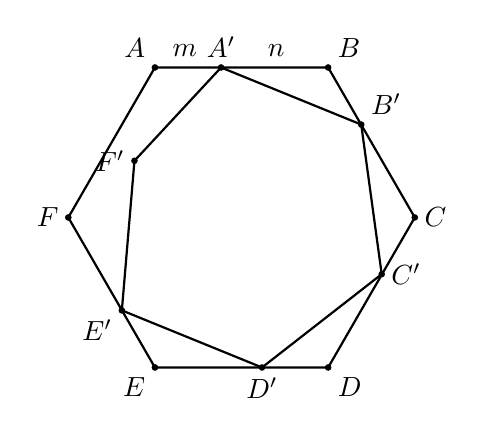
\begin{tikzpicture}[scale=1.0]
  \coordinate (A) at (-1.1,1.905);
  \coordinate (B) at (1.1,1.905);
  \coordinate (C) at (2.2,0);
  \coordinate (D) at (1.1,-1.905);
  \coordinate (E) at (-1.1,-1.905);
  \coordinate (F) at (-2.2,0);
  \coordinate (Ap) at (-0.26,1.905);
  \coordinate (Bp) at (1.52,1.18);
  \coordinate (Cp) at (1.78,-0.72);
  \coordinate (Dp) at (0.26,-1.905);
  \coordinate (Ep) at (-1.52,-1.18);
  \coordinate (Fp) at (-1.36,0.72);
  \draw[thick] (A)--(B)--(C)--(D)--(E)--(F)--cycle;
  \draw[thick] (Ap)--(Bp)--(Cp)--(Dp)--(Ep)--(Fp)--cycle;
  \fill (A) circle (1.2pt) node[above left] {$A$};
  \fill (B) circle (1.2pt) node[above right] {$B$};
  \fill (C) circle (1.2pt) node[right] {$C$};
  \fill (D) circle (1.2pt) node[below right] {$D$};
  \fill (E) circle (1.2pt) node[below left] {$E$};
  \fill (F) circle (1.2pt) node[left] {$F$};
  \fill (Ap) circle (1.2pt) node[above] {$A'$};
  \fill (Bp) circle (1.2pt) node[above right] {$B'$};
  \fill (Cp) circle (1.2pt) node[right] {$C'$};
  \fill (Dp) circle (1.2pt) node[below] {$D'$};
  \fill (Ep) circle (1.2pt) node[below left] {$E'$};
  \fill (Fp) circle (1.2pt) node[left] {$F'$};
  \node at (-0.72,2.12) {$m$};
  \node at (0.44,2.12) {$n$};
\end{tikzpicture}
\end{center}
\nopagebreak[4]
\begin{gktip}
\textbf{附加题}（原卷注明：满分 20 分，在 100 分之外，计入总分）
\end{gktip}

\textbf{附加题 1．} 已知 $\operatorname{Cos}\alpha+\operatorname{Sin}\alpha=\dfrac1{\sqrt2}$。试求：

（1） $\operatorname{Sin}^4\alpha+\operatorname{Cos}^4\alpha$；

（2） $\operatorname{Sin}^5\alpha+\operatorname{Cos}^5\alpha$。

\textbf{附加题 2．}

（1） 若 $a_i>0$（$i=1,2,\cdots,n$），证明：$\sum_{i=1}^{n}a_i\cdot\sum_{i=1}^{n}\frac1{a_i}\ge n^2$；

（2） 若 $f(x)$ 在 $[0,1]$ 上连续，且 $f(x)>0$，证明 $\int_0^1 f(x)\,dx\int_0^1\frac{dx}{f(x)}\ge 1$。

\begin{gktip}
\textbf{源注}：附加题 2(1) 题干中「$a_i>0$」后的括号在原卷排印为闭括号（原样为「$a_i>0$）$i=1,2,\cdots,n$）」），本库按开括号理解转录，未增删题干内容。
\end{gktip}

\end{question}